\chapter{TÍNH TOÁN, THIẾT KẾ HỆ THỐNG ĐIỆN}
    \section{Thiết kế sơ đồ nguyên lý điện}
        \begin{figure}[H]
            \centering
            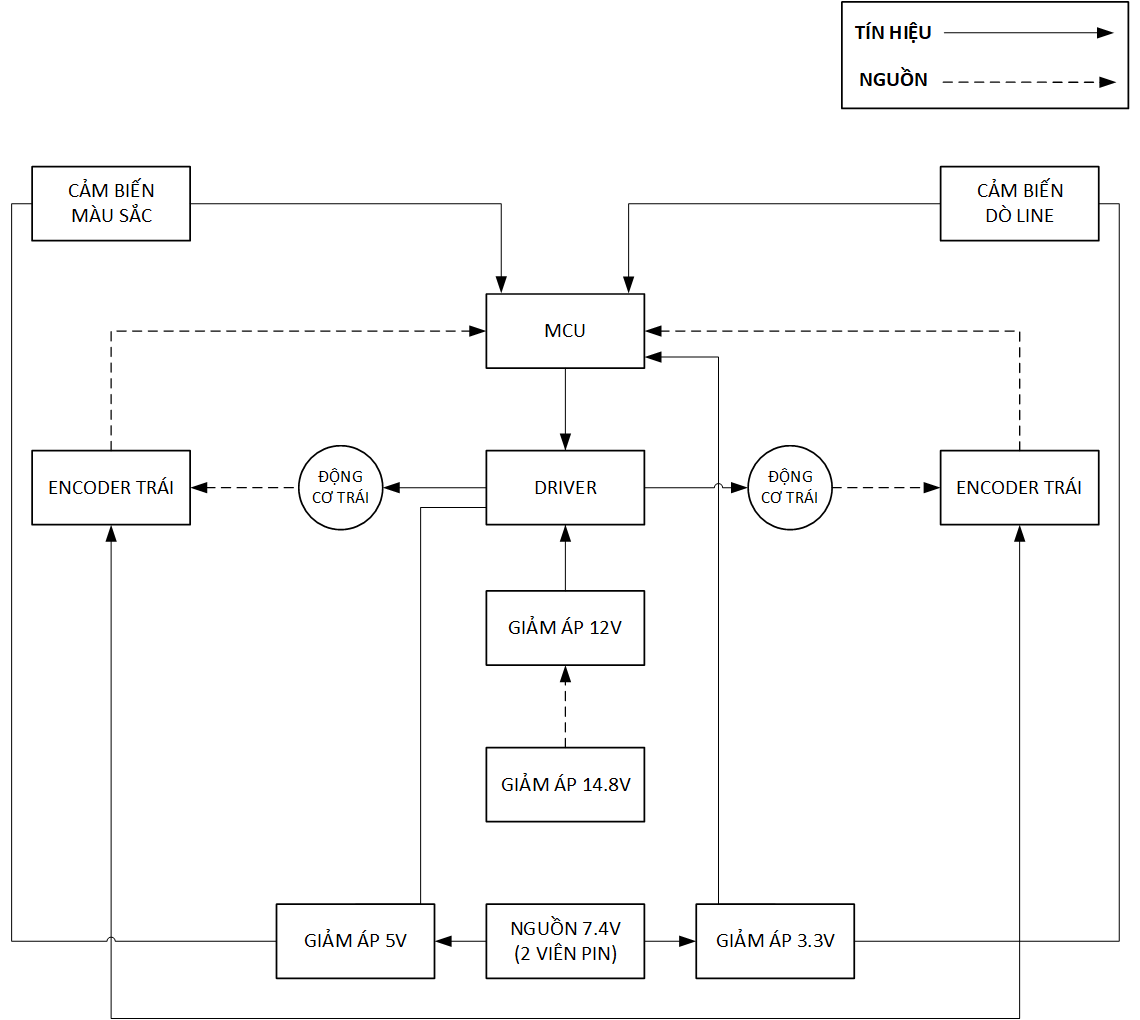
\includegraphics[width=1\textwidth]{pictures/chapter4/c4_p1_ElectricalFlow.png}
            \caption{Sơ đồ nguyên lý điện của hệ thống}
            \label{fig:4-1}
        \end{figure}
    \section{Thiết kế mạch cảm biến}
        \begin{figure}[H]
            \centering
            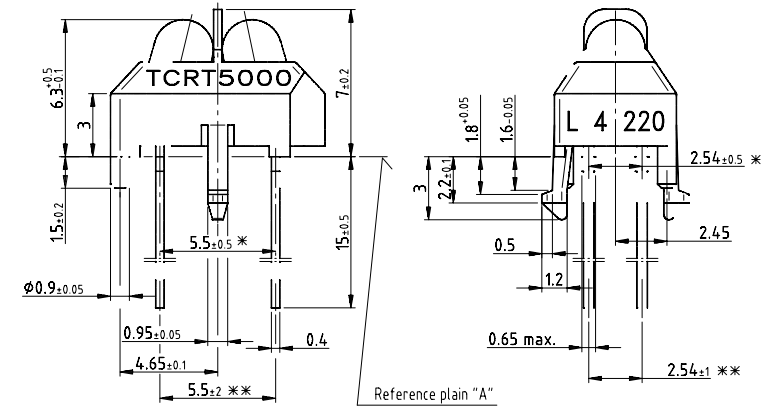
\includegraphics[width=1\textwidth]{pictures/chapter4/c4_p10_TCRT5000Dimensions1.png}
            \label{fig:4-2}
            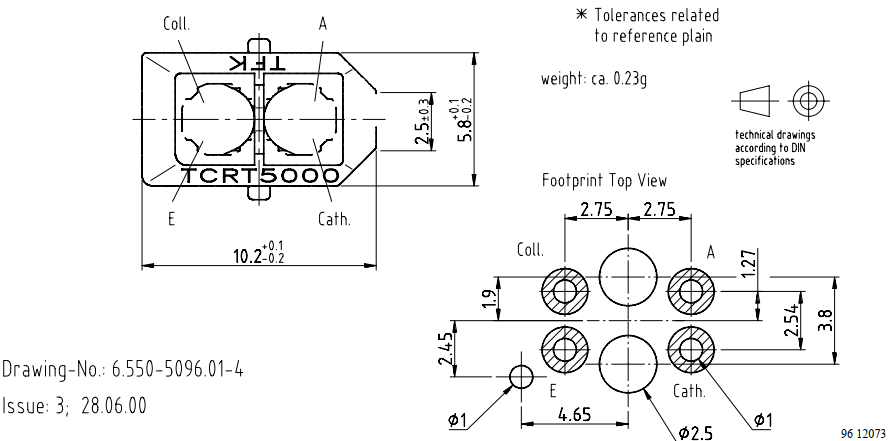
\includegraphics[width=1\textwidth]{pictures/chapter4/c4_p11_TCRT5000Dimensions2.png}
            \label{fig:4-3}
            \caption{Kích thước cảm biến TCRT5000}
        \end{figure}
        \hspace*{0.6cm}Theo tài liệu tham khảo \cite{vishay_tcrt5000_1}, ta có bảng đặc tính kỹ thuật của cảm biến TCRT5000 như sau:
        \begin{table}[H]
            \centering
            \begin{tabular}{|c|c|}
                \hline
                \textbf{Thông số} & \textbf{Giá trị} \\
                \hline
                Khoảng cách hoạt động & 0.2 - 15 (mm) \\
                \hline
                Kích thước bao & 10.2 x 5.8 x 7 (mm) \\
                \hline
                Góc phát & $16^{\circ}$ \\
                \hline
                Góc thu & $30^{\circ}$ \\
                \hline
                $I_{C}$ (max) & 100 (mA) \\
                \hline
                $I_{F}$ (max) & 60 (mA) \\
                \hline
            \end{tabular}
            \caption{Đặc tính kỹ thuật của cảm biến TCRT5000}
            \label{tab:4-1}
        \end{table}
        \subsection{Tính chọn điện trở cho cảm biến dò line}
            \begin{figure}[H]
                \centering
                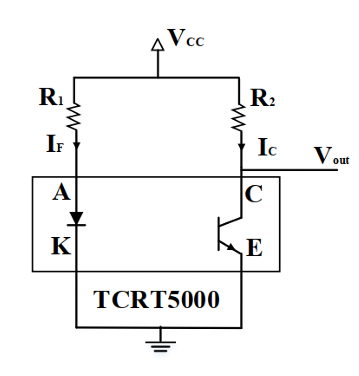
\includegraphics[width=0.35\textwidth]{pictures/chapter4/c4_p2_TCRT5000Schematic.png}
                \caption{Sơ đồ mạch điện TCRT5000}
                \label{fig:4-4}
            \end{figure}
            \hspace*{0.6cm}Dựa vào đường đặc tuyến trên datasheet, ta chọn $V_{F} = 1.1$ (V) và $I_{F} = 10$ (mA).\\
            \begin{figure}[H]
                \centering
                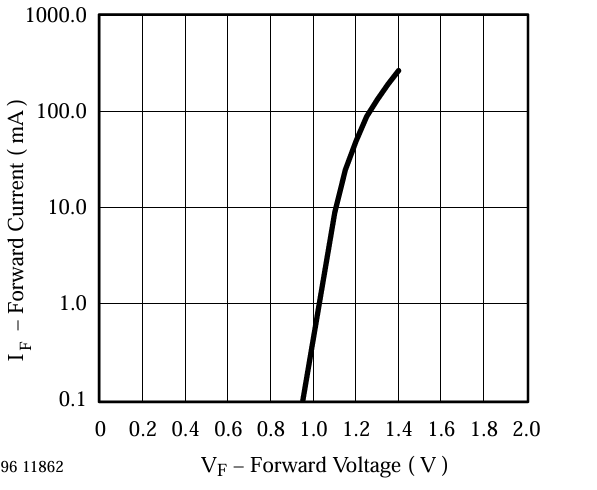
\includegraphics[width=0.5\textwidth]{pictures/chapter4/c4_p3_Voltage&Current.png}
                \caption{Đường đặc tuyến $V_{F}$ và $I_{F}$ của TCRT5000}
                \label{fig:4-5}
            \end{figure}
            Để tính điện trở R1, ta sử dụng công thức:
            \begin{equation}
                R_{1} = \frac{V_{CC} - V_{F}}{I_{F}} = \frac{3.3 - 1.1}{0.01} = 220 \Omega
                \label{eq:4-1}
            \end{equation}
            \hspace*{0.6cm}Chọn điện trở R1 là $220 \Omega$ theo tiêu chuẩn trên thị trường.\\[0.4cm]
            \hspace*{0.6cm}Từ đường đặc tuyến $I_{C} - I_{F}$. Với $I_{F} = 10$ (mA) $\Rightarrow$ $I_{C} \approx 1$ (mA).
            \begin{figure}[H]
                \centering
                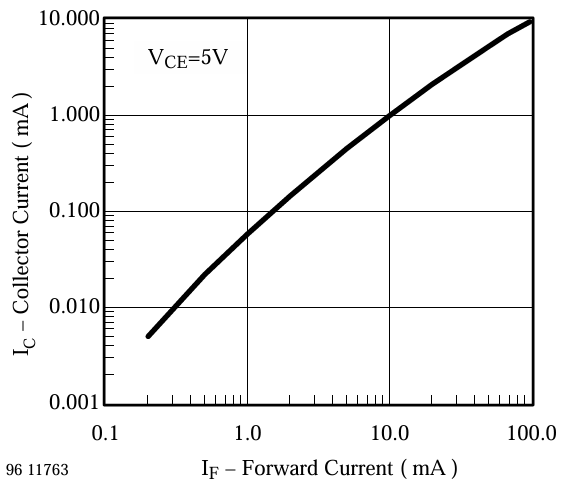
\includegraphics[width=0.5\textwidth]{pictures/chapter4/c4_p4_IC&IF.png}
                \caption{Đường đặc tuyến $I_{C}$ và $I_{F}$ của TCRT5000}
                \label{fig:4-6}
            \end{figure}
            Từ đường đặc tuyến $V_{CE} - I_{C} - I_{F}$, với $I_{C} = 1$ (mA) và $I_{F} = 10$ (mA) $\Rightarrow$ $V_{CE} \approx 1$ (V).\\
            \begin{figure}[H]
                \centering
                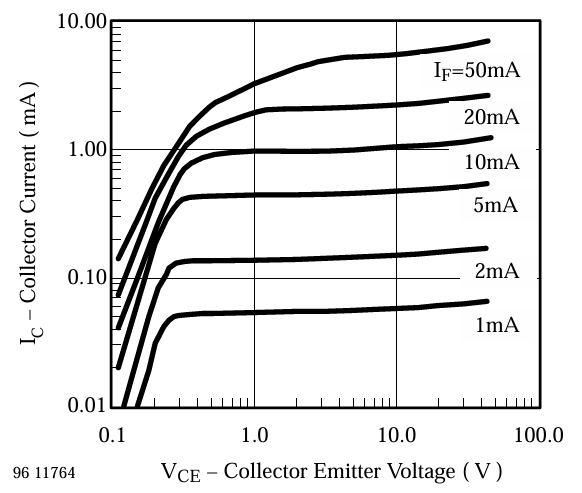
\includegraphics[width=0.5\textwidth]{pictures/chapter4/c4_p5_VCE&IC&IF.png}
                \caption{Đường đặc tuyến $V_{CE}$, $I_{C}$ và $I_{F}$ của TCRT5000}
                \label{fig:4-7}
            \end{figure}
            Từ đó, ta tính điện trở R2:
            \begin{equation}
                R_{2} = \frac{V_{CC} - V_{CE}}{I_{C}} = \frac{3.3 - 1}{0.001} = 2300 \Omega
                \label{eq:4-2}
            \end{equation}
            \hspace*{0.6cm}Chọn điện trở R2 là $2.4 k\Omega$ theo tiêu chuẩn trên thị trường.\\[0.4cm]
        \subsection{Xác định cách đặt cảm biến}
            \hspace*{0.6cm}Có 2 cách đặt cảm biến dò line:
            \begin{itemize}
                \item Trục giữa của bộ phát (S) và thu (E) vuông góc với biên phân cách sáng – tối (Position 1).
                \item Trục giữa của bộ phát (S) và thu (E) song song với biên phân cách sáng – tối (Position 2).
            \end{itemize}
            \begin{figure}[H]
                \centering
                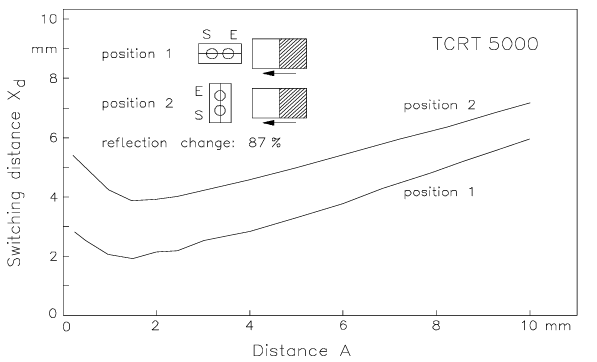
\includegraphics[width=0.8\textwidth]{pictures/chapter4/c4_p6_SensorPosition.png}
                \caption{So sánh độ phân giải của cảm biến khi đặt ở 2 vị trí khác nhau}
                \label{fig:4-8}
            \end{figure}
            \hspace*{0.6cm}Từ hình trên, ta thấy vị trí đặt cảm biến như Position 1 sẽ cho độ phân giải cao hơn so với Position 2. Do đó, ta chọn cách đặt cảm biến ở Position 1.
        \subsection{Xác định khoảng cách giữa cảm biến dò line và sa bàn}
            \hspace*{0.6cm}Theo datasheet, trong khoảng cách từ 0.2 - 15 mm thì cảm biến cho kết quả tốt nhất. Do đó tiến hành đo giá trị ADC từ cảm biến trong khoảng 1 - 15mm trên sa bản và thu được kết quả.
            \begin{table}[H]
                \centering
                \begin{tabular}{|c|c|c|c|}
                    \hline
                    \textbf{h (mm)} & \textbf{Giá trị vùng trắng} & \textbf{Giá trị vùng đen} & \textbf{Chênh lệch} \\
                    \hline
                    1 & 39 & 814 & 775 \\
                    \hline
                    2 & 37 & 798 & 761 \\
                    \hline
                    3 & 37 & 785 & 748 \\
                    \hline
                    4 & 34 & 786 & 752 \\
                    \hline
                    5 & 36 & 793 & 757 \\
                    \hline
                    6 & 37 & 797 & 760 \\
                    \hline
                    7 & 36 & 804 & 768 \\
                    \hline
                    \rowcolor{yellow!50}
                    8 & 38 & 841 & 803 \\
                    \hline
                    \rowcolor{yellow!50}
                    9 & 39 & 856 & 817 \\
                    \hline
                    \rowcolor{yellow!50}
                    10 & 40 & 864 & 824 \\
                    \hline
                    \rowcolor{yellow!50}
                    11 & 41 & 878 & 837 \\
                    \hline
                    \rowcolor{yellow!50}
                    12 & 53 & 894 & 841 \\
                    \hline
                    13 & 134 & 872 & 738 \\
                    \hline
                    14 & 162 & 936 & 774 \\
                    \hline
                    15 & 231 & 896 & 665 \\
                    \hline
                \end{tabular}
                \caption{Giá trị ADC từ cảm biến dò line ở các khoảng cách khác nhau}
            \end{table}
            \begin{figure}[H]
                \centering
                \begin{tikzpicture}
                    \begin{axis}[
                        width=14cm,
                        height=8cm,
                        xlabel={Khoảng cách h (mm)},
                        ylabel={Giá trị ADC},
                        legend pos=north west,
                        grid=major,
                        xmin=0, xmax=16,
                        ymin=0, ymax=1000,
                        mark size=2pt
                    ]
                    
                    % Đường giá trị vùng trắng
                    \addplot[color=blue, mark=o, thick] coordinates {
                        (1,39) (2,37) (3,37) (4,34) (5,36) (6,37) (7,36) 
                        (8,38) (9,39) (10,40) (11,41) (12,53) (13,134) 
                        (14,162) (15,231)
                    };
                    \addlegendentry{Vùng trắng}
                    
                    % Đường giá trị vùng đen
                    \addplot[color=red, mark=square, thick] coordinates {
                        (1,814) (2,798) (3,785) (4,786) (5,793) (6,797) (7,804) 
                        (8,841) (9,856) (10,864) (11,878) (12,894) (13,872) 
                        (14,936) (15,896)
                    };
                    \addlegendentry{Vùng đen}
                    
                    % Highlight vùng tối ưu (8-12mm)
                    \addplot[color=gray, fill=yellow, fill opacity=0.3, draw=none] 
                    coordinates {(8,0) (8,1000) (12,1000) (12,0)} \closedcycle;
                    
                    \end{axis}
                \end{tikzpicture}
                \caption{Đồ thị giá trị ADC theo khoảng cách cảm biến}
                \label{fig:4.9}
            \end{figure}

            % Vẽ đồ thị chênh lệch
            \begin{figure}[H]
                \centering
                \begin{tikzpicture}
                    \begin{axis}[
                        width=14cm,
                        height=8cm,
                        xlabel={Khoảng cách h (mm)},
                        ylabel={Chênh lệch giá trị ADC},
                        grid=major,
                        xmin=0, xmax=16,
                        ymin=600, ymax=900,
                        mark size=2pt
                    ]
                    
                    % Đường chênh lệch
                    \addplot[color=green, mark=triangle, thick] coordinates {
                        (1,775) (2,761) (3,748) (4,752) (5,757) (6,760) (7,768) 
                        (8,803) (9,817) (10,824) (11,837) (12,841) (13,738) 
                        (14,774) (15,665)
                    };
                    
                    % Highlight vùng tối ưu
                    \addplot[color=gray, fill=green, fill opacity=0.2, draw=none] 
                    coordinates {(8,600) (8,900) (12,900) (12,600)} \closedcycle;
                    
                    \end{axis}
                \end{tikzpicture}
                \caption{Đồ thị chênh lệch giá trị ADC theo khoảng cách}
                \label{fig:4.10}
            \end{figure}
            Từ bảng trên ta thấy trong khoảng h từ 8 - 12 mm thì chênh lệch giá trị ADC giữa vùng trắng và vùng đen là lớn nhất và ổn định nhất. Do đó, ta tiếp tục cho cảm biến đi ngang qua đường line với quãng đường 20mm quanh ranh giới trắng và đen trong khoảng h từ 8 - 12 mm để xác định độ cao thích hợp nhất.
                \begin{table}[H]
            \centering
            \begin{tabular}{|c|c|c|c|c|c|c|c|c|c|c|c|}
                \hline
                \textbf{h} & \textbf{0} & \textbf{1} & \textbf{2} & \textbf{3} & \textbf{4} & \textbf{5} & \textbf{6} & \textbf{7} & \textbf{8} & \textbf{9} & \textbf{10} \\
                \hline
                \textbf{8} & 45 & 44 & 54 & 135 & 200 & 285 & 345 & 491 & 623 & 655 & 713 \\
                \hline
                \textbf{9} & 43 & 43 & 52 & 130 & 190 & 280 & 340 & 503 & 625 & 662 & 721 \\
                \hline
                \textbf{10} & 45 & 43 & 52 & 93 & 195 & 277 & 332 & 505 & 609 & 674 & 739 \\
                \hline
                \textbf{11} & 43 & 43 & 50 & 112 & 189 & 263 & 349 & 482 & 615 & 663 & 698 \\
                \hline
                \textbf{12} & 41 & 40 & 44 & 90 & 167 & 233 & 313 & 473 & 591 & 639 & 679 \\
                \hline
            \end{tabular}
        \end{table}

        \begin{table}[H]
            \centering
            \begin{tabular}{|c|c|c|c|c|c|c|c|c|c|c|}
                \hline
                \textbf{h} & \textbf{11} & \textbf{12} & \textbf{13} & \textbf{14} & \textbf{15} & \textbf{16} & \textbf{17} & \textbf{18} & \textbf{19} & \textbf{20} \\
                \hline
                \textbf{8} & 790 & 819 & 850 & 855 & 865 & 870 & 855 & 878 & 875 & 877 \\
                \hline
                \textbf{9} & 785 & 823 & 845 & 850 & 860 & 865 & 850 & 873 & 870 & 872 \\
                \hline
                \textbf{10} & 794 & 836 & 848 & 853 & 863 & 863 & 862 & 862 & 860 & 863 \\
                \hline
                \textbf{11} & 787 & 825 & 857 & 861 & 867 & 873 & 877 & 877 & 875 & 876 \\
                \hline
                \textbf{12} & 765 & 803 & 825 & 836 & 844 & 849 & 849 & 852 & 857 & 855 \\
                \hline
            \end{tabular}
            \caption{Giá trị ADC khi cảm biến đi qua đường line với khoảng cách khác nhau}
            \label{tab:sensor-spacing-adc}
        \end{table}

        \begin{figure}[H]
            \centering
            \begin{tikzpicture}
                \begin{axis}[
                    width=16cm,
                    height=10cm,
                    xlabel={Vị trí cảm biến (mm)},
                    ylabel={Giá trị ADC},
                    legend pos=north west,
                    grid=major,
                    xmin=-1, xmax=21,
                    ymin=0, ymax=1000,
                    mark size=1.5pt,
                    legend style={font=\small}
                ]
                
                % h = 8mm (màu xanh dương)
                \addplot[color=blue, mark=none, thick, smooth] coordinates {
                    (0,45) (1,44) (2,54) (3,135) (4,200) (5,285) (6,345) (7,491) (8,623) (9,655) 
                    (10,713) (11,790) (12,819) (13,850) (14,855) (15,865) (16,870) (17,855) (18,878) (19,875) (20,877)
                };
                \addlegendentry{8}
                
                % h = 9mm (màu cam)
                \addplot[color=orange, mark=none, thick, smooth] coordinates {
                    (0,43) (1,43) (2,52) (3,130) (4,190) (5,280) (6,340) (7,503) (8,625) (9,662) 
                    (10,721) (11,785) (12,823) (13,845) (14,850) (15,860) (16,865) (17,850) (18,873) (19,870) (20,872)
                };
                \addlegendentry{9}
                
                % h = 10mm (màu đỏ - highlight)
                \addplot[color=red, mark=none, thick, smooth] coordinates {
                    (0,45) (1,43) (2,52) (3,93) (4,195) (5,277) (6,332) (7,505) (8,609) (9,674) 
                    (10,739) (11,794) (12,836) (13,848) (14,853) (15,863) (16,863) (17,862) (18,862) (19,860) (20,863)
                };
                \addlegendentry{10}
                
                % h = 11mm (màu vàng)
                \addplot[color=yellow!80!black, mark=none, thick, smooth] coordinates {
                    (0,43) (1,43) (2,50) (3,112) (4,189) (5,263) (6,349) (7,482) (8,615) (9,663) 
                    (10,698) (11,787) (12,825) (13,857) (14,861) (15,867) (16,873) (17,877) (18,877) (19,875) (20,876)
                };
                \addlegendentry{11}
                
                % h = 12mm (màu xanh nhạt)
                \addplot[color=cyan, mark=none, thick, smooth] coordinates {
                    (0,41) (1,40) (2,44) (3,79) (4,167) (5,233) (6,313) (7,473) (8,591) (9,639) 
                    (10,679) (11,765) (12,803) (13,825) (14,836) (15,844) (16,849) (17,849) (18,852) (19,857) (20,855)
                };
                \addlegendentry{12}
                
                % Đánh dấu vị trí chuyển line tại x = 10
                \addplot[color=black, mark=none, thick, dashed] coordinates {(10,0) (10,1000)};
                
                % Thêm text đánh dấu
                \node[anchor=south] at (axis cs:10,900) {\textbf{Chuyển line}};
                \node[anchor=south] at (axis cs:10,850) {\textbf{(Vị trí 10)}};
                
                % Đánh dấu vùng trước và sau line
                \node[anchor=center] at (axis cs:5,600) {\textbf{Vùng trắng}};
                \node[anchor=center] at (axis cs:15,600) {\textbf{Vùng đen}};
                
                \end{axis}
            \end{tikzpicture}
            \caption{Biểu đồ giá trị ADC khi cảm biến đi qua đường line}
            \label{fig:4-11}
        \end{figure}
        Từ bảng và đồ thị trên, ta thấy tại h = 10mm, cảm biến cho kết quả chuyển tiếp rõ ràng và nhanh nhất giữa nền trắng và nền đen. Do đó, ta chọn khoảng cách từ cảm biến dò line đến sa bàn là 10mm.

        \subsection{Xác định khoảng cách giữa các cảm biến}
            \begin{figure}[H]
                \centering
                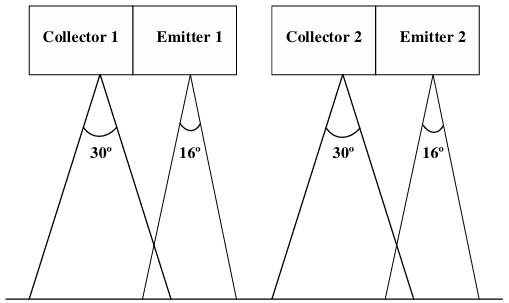
\includegraphics[width=0.7\textwidth]{pictures/chapter4/c4_p7_DistanceCollectorEmitter1.png}
                \label{fig:4-12}
                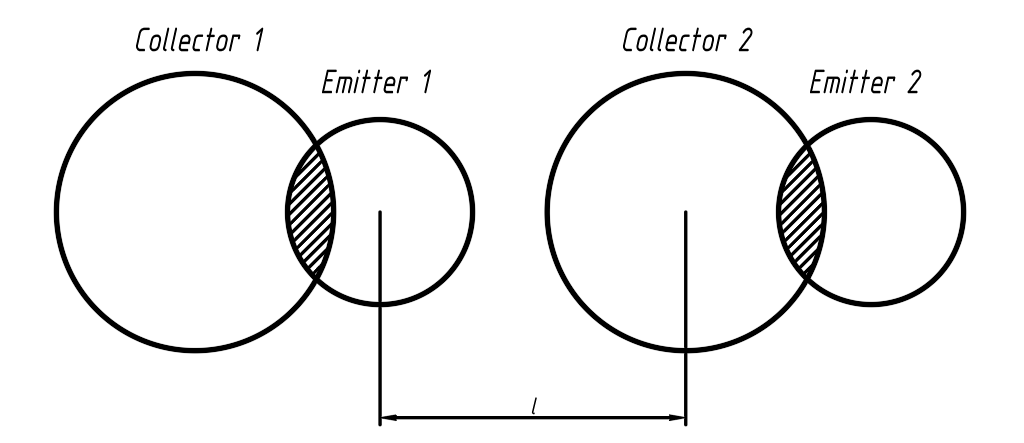
\includegraphics[width=0.8\textwidth]{pictures/chapter4/c4_p8_DistanceCollectorEmitter2.png}
                \caption{Khoảng cách giữa các vùng thu và vùng phát}
                \label{fig:4-13}
                \end{figure}
            \hspace*{0.6cm}Với h = 10mm, ta tính khoảng cách giữa vùng phát và vùng thu liền kề nhau tối thiểu để không bị giao thoa là:
            \begin{align}
                l_{min} &= (r + R) \label{eq:4-3} \\
                        &= (h +0.7) \cdot \tan{8^{\circ}} + (h + 0.7) \cdot \tan{15^{\circ}} \nonumber \\
                        &= (10 + 0.7) \cdot \tan{8^{\circ}} + (10 + 0.7) \cdot \tan{15^{\circ}} \nonumber \\
                        &= 4.4 \text{ (mm)} \nonumber
            \end{align}
            \hspace*{0.6cm}Khoảng cách tối thiểu giữa 2 cảm biến là:
            \begin{align}
                d_{min} = l_{min} + d = 4.4 + 3.8 = 8.2 \text{ (mm)}
                \label{eq:4-4}
            \end{align}
            \hspace*{0.6cm}Dựa vào datasheet, ta có chiều dài của cảm biến TCRT5000 là 10.2 mm (bố trí nằm ngang). Do đó, với độ cao $h = 10$ mm thì chắc chắn hai cảm biến liền kề không ảnh hưởng nhau.\\[0.4cm]
            \begin{figure}[H]
                \centering
                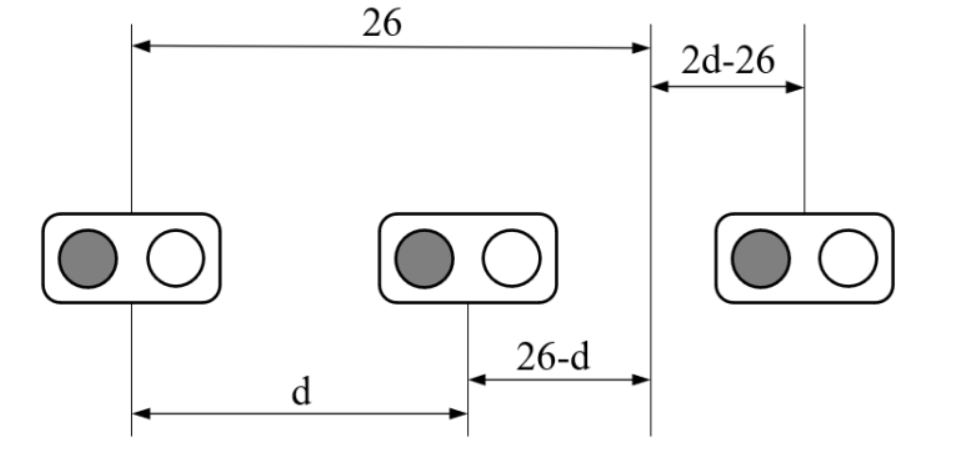
\includegraphics[width=0.8\textwidth]{pictures/chapter4/c4_p12_SensorDistance.png}
                \caption{Khoảng cách giữa các cảm biến dò line}
                \label{fig:4-14}
            \end{figure}
            Do line có bề rộng là 26mm nên tối đa có 3 cảm biến có vùng phát hiện nằm trong line. Bên cạnh đó, khi hoạt động sẽ có trường hợp cảm biến rơi vào vùng bất định thì giá trị analog trả về từ cảm biến sẽ như nhau. Do đó, không thể tính toán sai số để xác định được vị trí cảm biến so với đường tâm line. \\
            \hspace*{0.6cm}Ta xét các trường hợp:
            \begin{itemize}
                \item Trường hợp 1: Khi di chuyển sang phải trong khoảng 26 - d thì có 2 led nằm trong line nên thuđược giá trị analog là như nhau dẫn đến cảm biến rơi vào vùng bất định. 
                \item Trường hợp 2: Khi di chuyển sang trái trong khoảng 2d - 26 thì chỉ có 1 led nằm trên đường line và cũng rơi vào vùng bất định. 
            \end{itemize}
            \hspace*{0.6cm}Do đó để hạn chế việc cảm biến rơi vào vùng bất định thì lựa chọn khoảng cách $d$ sao cho $f_1 = 26 - d$ và $f_2 = 2d - 26$ là nhỏ nhất. \\
            \hspace*{0.6cm}Do $f_1$ là hàm đơn điệu giảm, $f_2$ là hàm đơn điệu tăng nên để $f_1$ và $f_2$ là nhỏ nhất thì ta chọn $f_1 = f_2$. Từ đó ta có:
            \begin{align}
                f_1 &= f_2 \label{eq:4-5}\\
                \Rightarrow 26 - d &= 2d - 26 \nonumber \\
                \Rightarrow d &= 17.33 \text{ (mm)} \nonumber
            \end{align}
        \subsection{Thiết kế sơ đồ nguyên lý mạch cảm biến}
            \hspace*{0.6cm}Dựa vào các tính toán trên, ta thiết kế sơ đồ nguyên lý mạch cảm biến như sau:
            \begin{itemize}
                \item Sử dụng 5 cảm biến TCRT5000 được bố trí nằm ngang vuông góc theo đường line.
                \item Khoảng cách từ cảm biến đến sa bàn là 10mm.
                \item Khoảng cách giữa các cảm biến là 17mm.
                \item Điện trở R1 là 220$\Omega$ và R2 là 2.4k$\Omega$.
            \end{itemize}
            \begin{figure}[H]
                \centering
                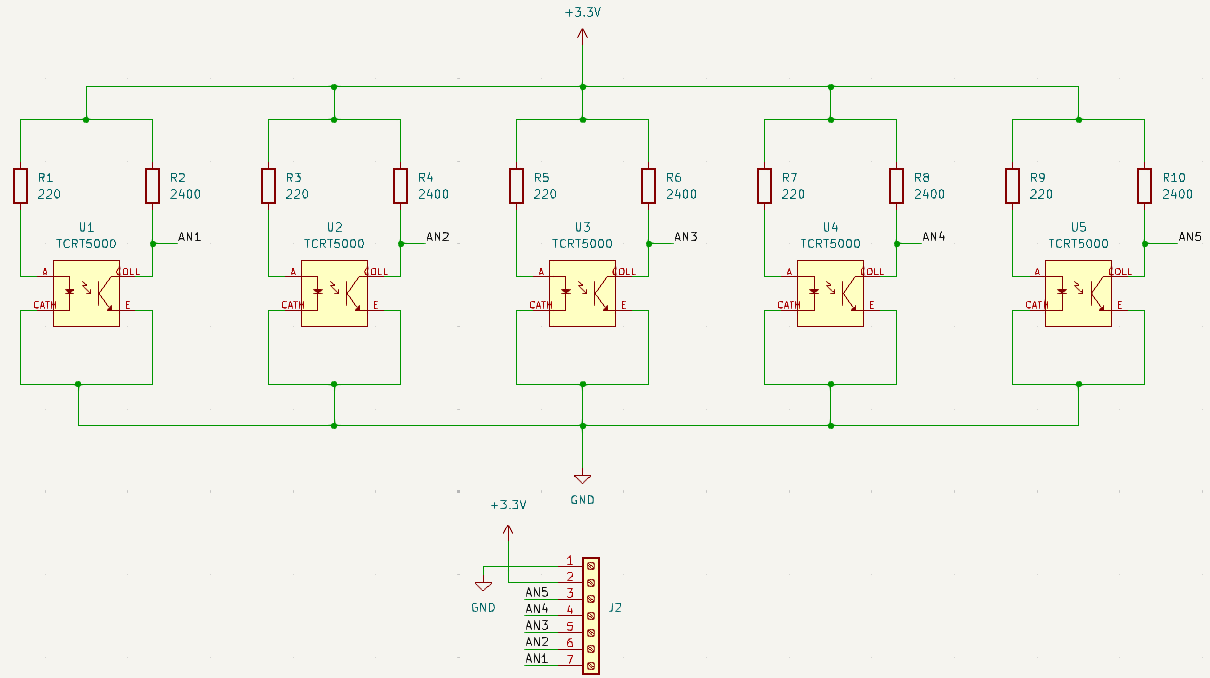
\includegraphics[width=1\textwidth]{pictures/chapter4/c4_p13_SensorSchematic.png}
                \caption{Sơ đồ nguyên lý mạch cảm biến dò line}
                \label{fig:4-15}
            \end{figure}
        \subsection{Thiết kế PCB mạch cảm biến}

            \hspace*{0.6cm}Dựa vào sơ đồ nguyên lý mạch cảm biến, ta tiến hành thiết kế PCB cho mạch cảm biến dò line. Sơ đồ thiết kế PCB được trình bày như hình \ref{fig:4-16}.

            \begin{figure}[H]
                \centering
                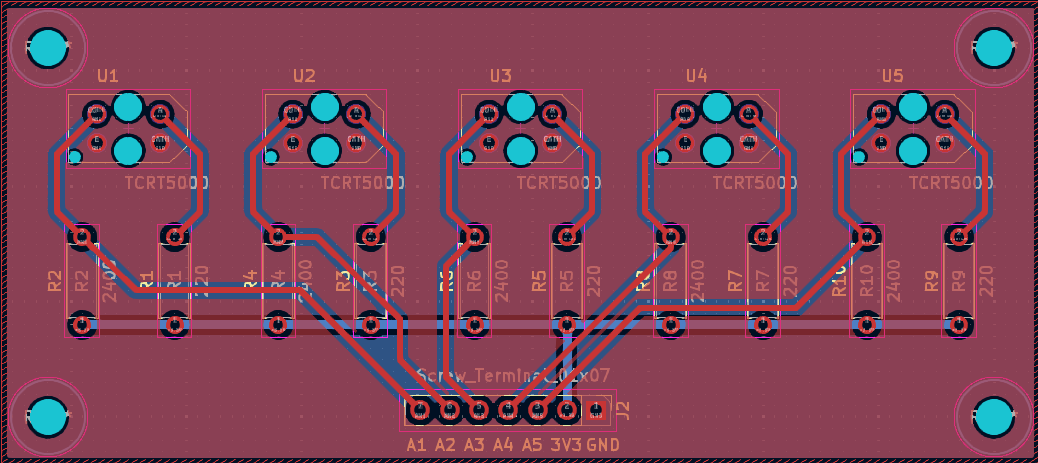
\includegraphics[width=1\textwidth]{pictures/chapter4/c4_p14_SensorPCB.png}
                \caption{Sơ đồ thiết kế PCB mạch cảm biến dò line}
                \label{fig:4-16}
            \end{figure}
        \subsection{Calib và tuyến tính hóa cảm biến}
            \hspace*{0.6cm}Mỗi cảm biến dò line sẽ trả về tín hiệu analog khác nhau trong cùng điều kiện. Do đó, việc calib cảm biến là vô cùng cần thiết. Lựa chọn phương pháp calib bằng công thức:
            \begin{align}
                y_i = y_{min} + \frac{(y_{max} - y_{min})(x_{max, i} - x_{min, i})}{x_{ij} - x_{min, i}} 
                \label{eq:4-6}
            \end{align}
            Trong đó:
            \begin{itemize}
                \item $x_{max,i}$ và $x_{min,i}$: giá trị analog lớn nhất và nhỏ nhất của cảm biến thứ $i$
                \item $y_{max}$ và $y_{min}$: giá trị analog lớn nhất và nhỏ nhất mà ta mong muốn cho tất cả cảm biến
                \item $x_{ij}$: giá trị analog đọc về từ cảm biến thứ $i$
                \item $y_{i0}$: giá trị analog đọc về sau khi đã calib của cảm biến thứ $i$
            \end{itemize}
            \begin{table}[H]
                \centering
                \begin{tabular}{|c|c|c|}
                    \hline
                    \textbf{Cảm biến} & $\mathbf{x_{max,i}}$ & $\mathbf{x_{min,i}}$  \\
                    \hline
                    Cảm biến 1 & 870 & 54  \\
                    \hline
                    Cảm biến 2 & 805 & 51  \\
                    \hline
                    Cảm biến 3 & 872 & 73  \\
                    \hline
                    Cảm biến 4 & 855 & 65  \\
                    \hline
                    Cảm biến 5 & 863 & 88  \\
                    \hline
                \end{tabular}
                \caption{Bảng giá trị analog của cảm biến trước khi calib ở độ cao h = 10mm}
                \label{tab:4-3}
            \end{table}